In order to complete the experiments, a few assumptions had to be made and are stated here.

\begin{itemize}
  \item The household being simulated was assumed to be "average", which means it uses 10,812 kWh of energy per year \cite{noauthor_how_nodate}. This works out to be just over 29 kWh per day.
  \item The household has a 5 kW solar panel array, which is reportedly the most common solar panel size in the US.
  \item The battery system is a Tesla Powerwall 2, with a 13.5 kWh capacity and a 5 kW max discharge/charge rate. It is also assumed that the battery is "perfect" and thus does not incur any parasitic loss while charging, discharging, or idling.
  \item The smart battery mainly looks 24 hours into the future before making a decision, though tests of 12 and 36 hours were also run.
  \item The home has an identical power curve every day, regardless of the time of year.
  \item The home is not able to take advantage of net metering, where excess energy can be "sold" back into the electrical grid in exchange for energy credits.
\end{itemize}

With this is mind, there were three experiments conducted using the simulator, with the potential for more at a future time.

\begin{itemize}
  \item \textbf{Experiment 1:} Examining yearly energy cost of the 8 possible combinations of technologies
  \item \textbf{Experiment 2:} Looking at the technologies in isolation
  \item \textbf{Experiment 3:} Exploring changes in yearly energy cost of looking ahead 12, 24, and 36 hours before making a decision
\end{itemize}

\subsection*{Experiment 1: Examining yearly energy cost of the 8 possible combinations of technologies}

For this experiment, 8 different simulations were run, each representing a unique combination of the 3 technologies being studied. Those simulations including a battery run 24 hours of predictions before making a decision. A cost is obtained for every hour of the day, and those costs are summed over all of 2016 to obtain the results found in Figure \ref{experiment_1}.

\begin{figure}
 \begin{center}
  \begin{tabular}{cc}
   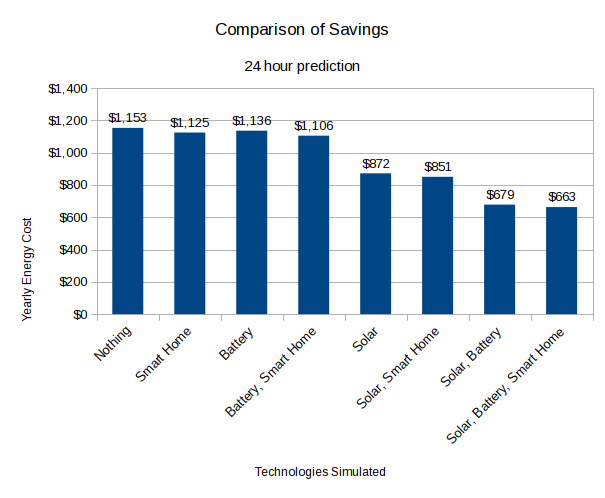
\includegraphics[width=0.50\textwidth]{./figures/experiment_1.png} \\
   \end{tabular}
   \end{center}
\caption{The results of simulating all combinations of technologies for all of year 2016}
  \vspace{+1mm}
\label{experiment_1}
\end{figure}

There are a few things of interest from these results.

First, it would appear that nearly negligible energy savings are to be found without solar. Even the battery, able to take advantage of cheaper energy prices, offers very little financial benefit. Solar immediately contributes 20-25\% savings in cost.

Another point of interest is that once you have solar, the battery becomes significantly more useful, saving an additional 15-20\% in energy costs. Thus, it can be seen that solar and a battery are superadditive, meaning the two technologies together contribute greater savings than the sum of their individual potential savings.

Finally, it would appear that the smart home, as represented in this study as shifting loads to off-peak times, contributes very little, even when coupled with solar and/or a battery.

\subsection*{Experiment 2: Looking at the technologies in isolation}

The next experiment considers each technology in isolation, showing the overall cost of all simulations that include a technology, compared to all simulations that did not include a technology. These results are found in Figure \ref{experiment_2}.

\begin{figure}
 \begin{center}
  \begin{tabular}{cc}
   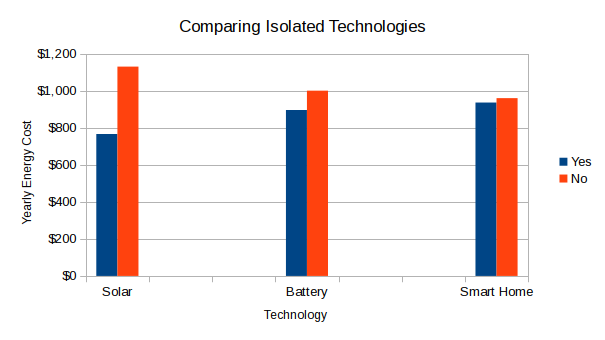
\includegraphics[width=0.50\textwidth]{./figures/experiment_2.png} \\
   \end{tabular}
   \end{center}
\caption{The results of isolating each technology}
  \vspace{+1mm}
\label{experiment_2}
\end{figure}

These results suggest that all technologies do contribute something in energy cost savings. As found in the previous experiment, solar contributes the most, with battery being the next greatest contributor. These results do suggest that smart home technology does contribute some to energy savings, though the contribution is so small as to hardly justify the expense of installing and maintaining such technologies.

\subsection*{Experiment 3: Exploring changes in yearly energy cost of looking ahead 12, 24, and 36 hours before making a decision}

This final experiment focuses more on the algorithm used to make a battery decision. As discussed previously, the Monte Carlo tree search algorithm used in this paper terminates a simulation after a specific number of hours in the future. The previous results used a fixed number of 24 hours in the future. This experiment runs the same simulation for all of year 2016, but terminates a battery simulation at times of 12, 24, and 36 hours in the future. These results are contained in Figure \ref{experiment_3}.

\begin{figure}
 \begin{center}
  \begin{tabular}{cc}
   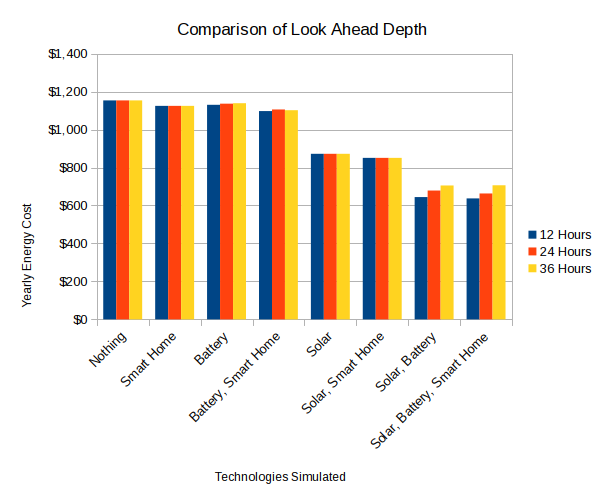
\includegraphics[width=0.50\textwidth]{./figures/experiment_3.png} \\
   \end{tabular}
   \end{center}
\caption{The results of allowing the battery to look 12, 24, and 36 hours into the future before making a decision}
  \vspace{+1mm}
\label{experiment_3}
\end{figure}

Of course the results with no battery are identical. However, when the battery is introduced alongside solar, there can be seen minor reductions in energy costs as simulation depth is reduced. These results are significant because this is a "free" upgrade, meaning it did not require any additional investments in hardware, only a modification to the algorithm running on already present hardware.

There are a few things that might explain these results. If you run the exact same simulation repeatedly, you will find that the battery does not always choose the same action, but instead chooses amongst several similar actions. Thus, in 10 runs of the simulator for the same hour, you might find several "c10", several "c20", and several "idle", meaning the battery chooses to charge at 10\% of the max rate, 20\% of the max rate, or idle. While these differences might be nearly insignificant in the period of 1 hour, over the course of a year the difference between charging at 10\% and 20\% can add up to a meaningful amount. When you run the simulation looking ahead only 12 hours, the algorithm can be more confident in a final decision as there is less variability in the end result. As you increase the search depth, there will be more variability in the end result, which may make deciding what to do now more difficult and prone to error.

Allowing the Monte Carlo tree search algorithm to run more simulations or simulate for a longer time might allow the results of 24 or 36 hour predictions to normalize with those of 12 hour predictions. However, more work would need to be done to understand if looking ahead that far is every advantageous. If you can always obtain results simply as good as 12 hours but not necessarily better, then there is no need to simulate beyond 12 hours. Perhaps simulating less than 12 hours ahead might be even more useful. These are all areas for further study.